\chapter{Methodology}
\label{chap:Three}

This chapter outlines the systematic approach taken to build the "Truth Scanner"—a neuro-symbolic pipeline that translates informal English mathematical definitions and theorems from textbooks into formally verified Lean 4 code. The methodology follows a three-phase research plan: Learning, Implementation (Translation), and Evaluation (Repair Loop).

\section{Overview of the Neuro-Symbolic Pipeline}
\label{sec:pipeline-overview}

The "Truth Scanner" operates as a Rosetta Stone for mathematics, bridging the gap between ambiguous human language and strict machine logic. The pipeline consists of two complementary components:

\begin{itemize}
    \item \textbf{Neuro Component (LLM)}: Handles the creative decomposition of informal English text into logical lemmas, leveraging Large Language Models to parse ambiguous natural language.
    \item \textbf{Symbolic Component (Lean 4 Kernel)}: Provides rigorous verification through the Lean 4 theorem prover, acting as the definitive validation mechanism that eliminates hallucinations and ensures mathematical correctness.
\end{itemize}

This dual-system approach addresses the fundamental challenge of auto-formalization: converting subtle, context-dependent human mathematical prose into unambiguous, machine-checkable formal proofs.

\begin{figure}[h]
\centering
\resizebox{\linewidth}{!}{%
\begin{tikzpicture}[node distance=2cm]
\node (input) [rectangle, draw, align=center, minimum width=2.5cm, minimum height=1cm] {Informal English\\(Textbook)};
\node (process) [rectangle, rounded corners, draw, align=center, right=of input, minimum width=3.5cm, minimum height=1cm, fill=blue!10] {LLM Translation\\(Neuro)};
\node (verify) [rectangle, draw, align=center, right=of process, minimum width=3.5cm, minimum height=1cm, fill=green!10] {Lean 4 Verifier\\(Symbolic)};
\node (output) [rectangle, draw, align=center, right=of verify, minimum width=2.5cm, minimum height=1cm] {Verified Proof\\(Formal Logic)};

\draw [->, thick] (input) -- (process);
\draw [->, thick] (process) -- (verify);
\draw [->, thick] (verify) -- (output);
\end{tikzpicture}%
}
\caption{High-Level Architecture of the Neuro-Symbolic Pipeline}
\label{fig:pipeline_arch}
\end{figure}

\section{Phase 1: Learning and Environment Setup}
\label{sec:phase1-learning}

\subsection{Lean 4 Environment Configuration}
The first phase established the technical foundation required for formal verification work. The development environment consisted of:

\begin{itemize}
    \item \textbf{Lean 4 Theorem Prover}: Installation and configuration of the Lean 4 proof assistant with the latest stable release.
    \item \textbf{VS Code Integration}: Setup of the Lean 4 VS Code extension for real-time proof state visualization and error feedback.
    \item \textbf{Mathlib Library}: Integration of Mathlib, the community-driven library containing thousands of formalized mathematical theorems essential for undergraduate-level mathematics.
\end{itemize}

A "Hello World" proof was implemented to verify the environment functionality, ensuring the complete toolchain could compile and verify basic Lean 4 code.

\subsection{The Natural Number Game}
To gain practical proficiency in Lean 4's tactic-based proof system, the "Natural Number Game" was completed. This gamified tutorial systematically introduced:

\begin{itemize}
    \item \textbf{Fundamental Tactics}: Core proof techniques including \texttt{intro}, \texttt{exact}, \texttt{rw} (rewrite), and \texttt{induction}.
    \item \textbf{Peano Axioms}: Building natural numbers from first principles using dependent type theory.
    \item \textbf{Proof Construction}: Completing verified proof scripts for the Addition and Multiplication worlds, establishing intuition for formal reasoning in Lean's syntax.
\end{itemize}

This hands-on training was critical for understanding how Lean 4 transforms mathematical goals into verified states and how tactics manipulate the proof context.

\section{Phase 2: Selection and Taxonomy}
\label{sec:phase2-selection}

\subsection{Source Material}
The project targeted Kenneth H. Rosen's \textit{Discrete Mathematics and Its Applications}, a standard undergraduate textbook used globally. This text was selected because:

\begin{itemize}
    \item It represents typical informal mathematical presentation found in educational materials.
    \item It contains precise definitions that are candidates for formalization.
    \item Known ambiguities in textbooks of this type provide realistic test cases for the pipeline.
\end{itemize}

\subsection{Definition Selection Criteria}
A systematic review identified 10–15 key definitions and theorems from Discrete Mathematics chapters covering:

\begin{itemize}
    \item Set theory operations (union, intersection, complement)
    \item Relations and functions
    \item Basic logic and propositional calculus
    \item Graph theory fundamentals
\end{itemize}

Each selected definition was mapped to its corresponding logical components, creating a taxonomy document that served as the foundation for translation work. This mapping explicitly identified:

\begin{itemize}
    \item The English-language definition as stated in the textbook
    \item The underlying logical structure (quantifiers, connectives, predicates)
    \item Potential ambiguities or implicit assumptions
    \item Expected Lean 4 type signatures
\end{itemize}

\section{Phase 3: Manual Formalization}
\label{sec:phase3-manual}

The third phase involved manually translating the selected definitions from English into verified Lean 4 code. This manual baseline serves multiple purposes:

\begin{itemize}
    \item Establishes ground truth for evaluating automated LLM translations
    \item Identifies common translation patterns and challenges
    \item Provides verified examples for training prompt engineering
\end{itemize}

\subsection{Translation Process}
For each definition, the manual formalization followed a structured workflow:

\begin{figure}[h]
\centering
\begin{tikzpicture}[node distance=1.5cm, auto]
    \node (decomp) [rectangle, draw, align=center, fill=orange!10] {1. Decomposition\\(Identify Components)};
    \node (type) [rectangle, draw, below=of decomp, align=center, fill=orange!10] {2. Type Design\\(Map to Mathlib)};
    \node (impl) [rectangle, draw, below=of type, align=center, fill=orange!10] {3. Implementation\\(Write Lean Code)};
    \node (verify) [rectangle, draw, below=of impl, align=center, fill=green!10] {4. Verification\\(Compile \& Check)};
    
    \draw [->, thick] (decomp) -- (type);
    \draw [->, thick] (type) -- (impl);
    \draw [->, thick] (impl) -- (verify);
\end{tikzpicture}
\caption{Manual Formalization Workflow for Textbook Definitions}
\label{fig:manual_workflow}
\end{figure}

\begin{enumerate}
    \item \textbf{Decomposition}: Break down the English definition into atomic logical statements.
    \item \textbf{Type Signature Design}: Define appropriate Lean 4 types for mathematical objects (sets, functions, relations).
    \item \textbf{Implementation}: Write the Lean 4 definition using dependent types and Mathlib constructs.
    \item \textbf{Verification}: Ensure the Lean 4 compiler accepts the definition without errors.
    \item \textbf{Documentation}: Add comments mapping Lean constructs back to English phrases.
\end{enumerate}

\subsection{Deliverables}
The manual formalization phase produced:

\begin{itemize}
    \item A set of verified \texttt{.lean} files containing formalized definitions
    \item A document analyzing translation challenges and patterns
    \item Baseline metrics for code length and compilation success
\end{itemize}

These verified definitions serve as the gold standard for subsequent phases, where LLM-based automation will be evaluated against this manual baseline.

\section{Phase 4: Automated Pipeline and LLM Prompting}
\label{sec:phase4-pipeline}

With a baseline manually established, the focus of the pipeline transitioned to constructing the automated translation software. The goal of this phase was to develop an autonomous interface between an external Large Language Model (e.g., OpenAI's GPT-4) and the local Lean 4 ecosystem.

\subsection{Python Script Interface}
A generic Python command-line interface was constructed utilizing the \texttt{openai} Python library. The tool abstracts the underlying HTTP networking to directly accept plain English informal math texts via argument parsing and output the corresponding formal verification logic as `.lean` source files.

The translation logic relies on rigorous \textit{prompt engineering} to ensure formatting. The system prompt embedded in the script explicitly forbids markdown formatting, thereby guaranteeing the LLM's response only yields raw valid syntax, ready for immediate compilation by the mathematical symbol compiler.

\begin{figure}[H]
    \makebox[\textwidth][c]{%
        \IfFileExists{img/python_script_screenshot.png}{
            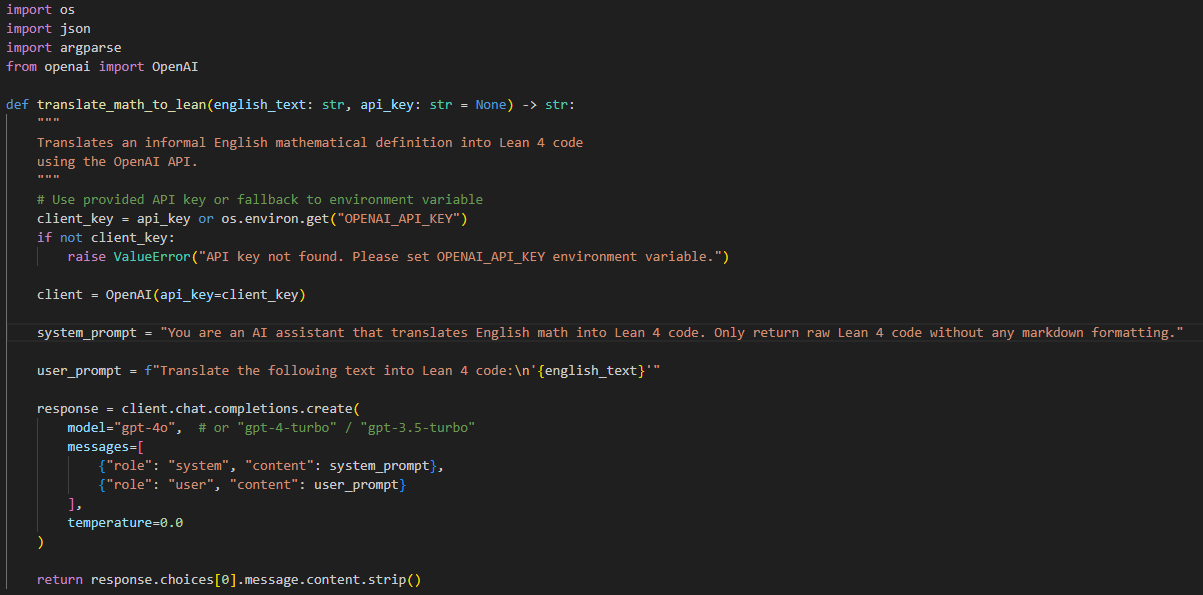
\includegraphics[width=1.2\textwidth]{img/python_script_screenshot.png}
        }{
            \fbox{\begin{minipage}[c][4cm][c]{1.2\textwidth}\centering Image: Python Script Interface (Placeholder, place 'python\_script\_screenshot.png' in img/ folder)\end{minipage}}
        }%
    }
    \caption{Core Prompt Logic from \texttt{llm\_translator.py}.}
    \label{fig:python-script}
\end{figure}

\subsection{Typing and Quantifier Enforcement}
Crucially, previous testing highlighted the LLM's poor habit of utilizing implicit type inference when auto-generating definitions. Without guidance, models frequently wrote raw natural definitions (e.g., $\forall x, x \in A$), leading to immediate compilation failures due to indeterminate universe structures. 
The Python prompt incorporates explicit system-level instructions demanding strict variable typing (such as coercing $\forall (x : \alpha)$ over sets), thus boosting first-pass compilation probability against Mathlib requirements.

\section{Phase 5: The Iterative Repair Loop and State-Space Formalization}
\label{sec:phase5-repair}

To transition from static auto-formalization to a dynamic theorem proving system, the pipeline mathematically requires an iterative feedback mechanism. When an initial translation $T_0$ fails to compile, the system enters a mathematically defined state-space to repair it.

\subsection{Mathematical Formalization of the Repair Mapping ($\Phi$)}
We systematically define the state-space of the repair agent as a tuple $(S, E, P)$, where:
\begin{itemize}
    \item $S$: The set of all possible Lean 4 abstract syntax trees (the formal code state).
    \item $E$: The set of all deterministic error bounds from the Lean 4 compiler (e.g., type mismatches, unknown identifiers).
    \item $P$: The domain of natural language correction prompts.
\end{itemize}

The formal mapping for the Error-to-Prompt transition is defined as:
\[ \Phi : E \times S \to P \]
This function $\Phi$ tokenizes the Lean compiler error $e_n \in E$ corresponding to code state $s_n \in S$ and translates it into a targeted LLM Correction Prompt $p_{n+1} \in P$. The model then yields a new state $s_{n+1}$, continuing until $e = \emptyset$ (successful compilation) or a maximum iteration threshold is reached.

\subsection{Implementation Procedures of the Repair Loop ($\Phi$ Mapping)}
To translate the mathematical framework of the repair mapping into a programmatic pipeline, the Python environment was heavily re-engineered to facilitate continuous dynamic feedback. The implemented algorithm operates iteratively via the following steps:
\begin{enumerate}
    \item \textbf{Initial Translation ($T_0$):} The LLM generates the first mathematical attempt at formalizing the English text via the OpenAI API.
    \item \textbf{Symbolic Audit ($D$):} The script captures the Lean 4 compiler output using the OS \texttt{subprocess} module. If the exit code matches $0$, the Verification Constraint is mathematically satisfied and the script finishes correctly.
    \item \textbf{Error Tokenization and Feedback Construction:} If the compilation fails, the script captures the standard error (\texttt{stderr}). A targeted \textit{Correction Prompt} is iteratively crafted, injecting the exact compiler traceback: \newline
    \textit{`The Lean 4 compiler returned the following error: <ERROR>. Please repair the code.`}
    \item \textbf{Message History Iteration ($T_{n+1}$):} The LLM receives the entire context tree (its previous failed translation and the Lean auditor's complaint) to output a repaired code block. The system iterates until $e = \emptyset$ or the operation exceeds a hard-coded failure bound.
\end{enumerate}

\begin{figure}[H]
    \centering
    \begin{tikzpicture}[
        node distance=1.5cm and 1cm,
        box/.style={rectangle, draw, rounded corners, minimum width=2.5cm, minimum height=1cm, text centered, text width=2.5cm, font=\small\sffamily},
        decision/.style={diamond, draw, aspect=1.8, text centered, text width=2.2cm, font=\small\sffamily},
        arrow/.style={thick, ->, >=stealth}
    ]

    % Nodes
    \node (input) [box] {1) User\\Math Input};
    \node (llm) [box, right=of input] {2) LLM\\Generator};
    \node (compiler) [decision, right=of llm] {3) Lean 4\\Compiler};
    \node (output) [box, right=of compiler] {Output};
    \node (truncator) [box, below=of compiler] {Context\\Truncator};

    % Arrows
    \draw [arrow] (input) -- (llm);
    \draw [arrow] (llm) -- (compiler);
    \draw [arrow] (compiler) -- node[anchor=south, font=\footnotesize] {YES} (output);
    \draw [arrow] (compiler) -- node[anchor=west, font=\footnotesize, align=left] {NO\\(Error)} (truncator);
    \draw [arrow] (truncator) -| node[anchor=north east, font=\footnotesize] {Filtered Prompt} (llm);

    \end{tikzpicture}
    \caption{Architecture of the Iterative Repair Loop ($\Phi$ Mapping), demonstrating the cyclic neuro-symbolic feedback.}
    \label{fig:repair-loop-arch}
\end{figure}

\subsection{Engineering Challenges and Ingenious Solutions}
During the implementation of the feedback loop, several practical software engineering challenges arose in bridging a probabilistic neuro-model with a strictly deterministic compiler:

\begin{itemize}
    \item \textbf{Context Window and Error Verbosity:} The Lean 4 compiler is notoriously verbose when throwing type-universe mismatches. Passing a multi-page traceback into the neuro-layer rapidly degraded the LLM's attention span, causing failure to identify the root syntax violation. \newline
    \textit{Solution:} The Python framework implements a strict "Context Window Truncation" bound ($E_{trunc}$). The prompt limits the traceback strictly to the first 1000 characters. This isolates the error tokenization to the exact mathematical violation without overloading the API sequence length.
    
    \item \textbf{Markdown Hallucination During Repair:} While the initial prompt accurately restricted the model to output raw code, during iterative \textit{correction} loops, the model frequently relapsed into "conversational apologies" or wrapped its repaired code in Markdown blocks (e.g., \texttt{```lean ... ```}). This predictably broke the subsequent compiler audit instantly. \newline
    \textit{Solution:} An ingenious programmatic "Sanitization Filter" was built directly into the Python loop pipeline. Before writing the state $s_{n}$ to the disk, the script rigorously searches for and strips any markdown bounding tags (and standard conversational filler) using string splits, guaranteeing that the Lean compiler purely parses verifiable math syntax.
    
    \item \textbf{Infinite Divergence Loops:} When the model fundamentally lacked the deep mathematical reasoning to repair a type structure, it would occasionally enter an infinite loop---rapidly alternating between two mathematically invalid states (e.g., oscillating between a missing universe mapping and incorrectly coercing the type parameter). \newline
    \textit{Solution:} The state-space exploration is explicitly bounded by a deterministic `max\_retries` counter (optimized to $N=5$). If $N$ is reached, the process gracefully aborts. The logical fallacy is then automatically diverted and documented into the fallback \textbf{Manual Auto-Formalization Benchmark}, preventing the execution cycle from crashing the pipeline entirely.
\end{itemize}

\subsection{Manual Auto-Formalization Benchmark (Fallback Paradigm)}
In instances where the structured repair loop reaches a technological dead-end (e.g., maximum iteration overload due to fundamental LLM reasoning logical fallacies), the protocol dictates a pivot to a \textbf{Manual Auto-Formalization Benchmark}. This acts as a robust measurement of the ``Repair Success Rate.'' Current model fallacies are strictly documented into categories (e.g., Type Inference Failure, Universe Instantiation Error, Hallucinated Tactic). Categorizing these specific logical fallacies, as identified by the Lean compiler auditor, ensures sustained scientific rigor across the thesis even when full automation yields false.
